% !TEX encoding = UTF-8 Unicode

%% Class options are described above.
\documentclass[subscriptcorrection,upint,varvw,mathalfa=cal=euler,barcolor=black,balance,hyphenate,french,pdf-a,nolists]{asmejour}

%% pdf metadata, the user should edit
\hypersetup{%
	pdftitle={Title of your paper},				% Write title of your project
	pdfkeywords={CFD, openFOAM, velocity, pressure},	% Write relevant keywords here
	pdfauthor={Chirag Trivedi},					% Write your name (First author only)
}

\JourName{TEP4545, Fluids Engineering}				% Journal/course name
\PreprintString{Preprint}						% Paper before peer-review

%% The default copyright year is the current year
%% \PaperYear{2020} sets 2020; and \PaperYear{} omits the year entirely.

\begin{document}
% Change to your author name[s] and addresses, in the desired order of authors.
% First name, middle initial, last name
% To label one or more corresponding authors put "Name\CorrespondingAuthor". No space after "Name".
% An optional argument can be added if email is not in address block as
%      "Name\CorrespondingAuthor{write@to.me}"
% Can also include multiple emails and use the command more than once for multiple corresponding authors,
%      "Name\CorrespondingAuthor{write@to.him, write@to.her}"

\SetAuthorBlock{Author Name 1\CorrespondingAuthor}
	{Department of Energy and Process Engineering,\\
	NTNU,\\
	Trondheim 7491, Norway \\
	email: \href{mailto:YourEmail@stud.ntnu.no}{YourEmail@stud.ntnu.no}}

\SetAuthorBlock{Author Name 2}
	{Department of Energy and Process Engineering,\\
	NTNU,\\
	Trondheim 7491, Norway \\
	email: \href{mailto:YourEmail@stud.ntnu.no}{YourEmail@stud.ntnu.no}}

\SetAuthorBlock{Author Name 3}
	{Department of Energy and Process Engineering,\\
	NTNU,\\
	Trondheim 7491, Norway \\
	email: \href{mailto:YourEmail@stud.ntnu.no}{YourEmail@stud.ntnu.no}}

\SetAuthorBlock{Author Name 4}
	{Department of Energy and Process Engineering,\\
	NTNU,\\
	Trondheim 7491, Norway \\
	email: \href{mailto:YourEmail@stud.ntnu.no}{YourEmail@stud.ntnu.no}}

%%% Change to your paper title. Can insert line breaks if you wish (otherwise breaks are selected automatically).
\title{Computational fluid dynamic analysis of flow over bluff body: Direct numerical simulation}

%%% Change these to your keywords.  Keywords are automatically printed at the end of the abstract.
%%% This command must come BEFORE the end of the abstract.
\keywords{CFD, openFOAM, velocity, pressure.}


%% Write abstract between \begin{abstract} and \end{abstract}
\begin{abstract}
Information about title: Select title of your project wisely, which must reflect your work clearly. Title should also reflect methodology and conclusion. Use sentence case title (exception for proper nouns). You must not use symbols or numbers in the title. Title must be smaller than 120 characters (with spacing) or 12 -- 15 words.

Abstract is a short summary of your work in 150 -- 200 words. More than 200 words are not permitted. The main purpose of an abstract is to contextualize and describe the work in a concise way and easily-understood manner. Read through the entire manuscript and distill your work to its main points or a short summary. You should write the abstract in the last, i.e., after completing all section and appendices. Potential reader from other engineering background can understand your work. Avoid usage of very specific and highly technical words. Clarity in writing is extremely important. Clarity is achieved by providing information in a predictable order.
\end{abstract}


\date{\today}%% You can modify this information as desired.
%% Putting \date{} will suppress any date.
%% If this command is omitted, date defaults to \today
%% This command must come somewhere before \maketitle

\maketitle %% This command creates the author/title/abstract block. Essential!

%%%%%%%%%%%%%%%%%%%%%%%%%%%%%%%%%%%%%%%%%%%%%%%%%%%%%%%%%%%%%%%%%%%%%%

\section{Introduction}
\label{sec:1}
Paper length must not exceed 10 pages, except appendix. It is relatively easy to write a long paper but, equally difficult to write a short version. The short version enables you to write only valuable and new information. Avoid jargon and information, which already exist in the giant ocean of internet. Presenting stuff, which can be found in common textbooks, will not give you added value. Structure of the paper between \ref{sec:1} Introduction and \ref{sec:4} Conclusion is flexible. Hence, you can decide what how to manage. Please remember, section headings are very important therefore select heading (name) wisely. Headings should reflect the content clearly.

After the abstract, a potential reader usually reads the introduction carefully to assess the importance and quality of the research undertaken. Introduction sets the background of your knowledge in the field. Introduction should be as simple as possible, even a reader from completely different field can understand what this work is about.The introduction shapes reader-expectations of what they will find by reading your work. In the initial paragraphs describes broad area of your discipline and the bigger challenge in the field. This helps reader to understand the engineering discipline your work. Then, critical summary of literature, which indicates the research gap and justification to select this problem, goal and objective of the work.

Selection of appropriate article indirectly indicates expertise and depth of knowledge you are presenting in the thesis. Use relevant keywords to search relevant journal articles. Use \href{https://scholar.google.com/}{google scholar} for global literature. Use \href{https://ntnuopen.ntnu.no/ntnu-xmlui/handle/11250/227455}{ntnu open} to find NTNU thesis. We usually find Majority of research articles from the following publishers/journals.

\begin{enumerate}
    \item \href{https://www.elsevier.com/}{Elsevier}
    \item \href{https://www.aip.org/}{American Institute of Physics}
    \item \href{https://www.cambridge.org/core/journals/journal-of-fluid-mechanics}{Journal of Fluid Mechanics}
    \item \href{https://www.tandfonline.com/}{Taylor and Francis}
    \item \href{https://asmedigitalcollection.asme.org/}{American Society of Mechanical Engineering}
    \item \href{https://www.asce.org/}{American Society of Civil Engineers}
    \item \href{https://www.mdpi.com/}{MDPI}
    \item \href{https://iopscience.iop.org/}{IOP Science} for conference papers.
\end{enumerate}

Close this section by writing main objective(s) and scope your work. Write a one or two sentence statement summarizing the conclusion you have reached after literature review. Introduction is usually 500 -- 700 words.

Recommended journals for literature
\begin{enumerate}
    \item \href{https://asmedigitalcollection.asme.org/fluidsengineering}{Fluids Engineering}
    \item \href{https://www.cambridge.org/core/journals/journal-of-fluid-mechanics}{Journal of Fluid Mechanics}
    \item \href{https://aip.scitation.org/journal/phf}{Physics of Fluids}
    \item \href{https://www.tandfonline.com/toc/tjhr20/current}{Journal of Hydraulic Research}
    \item \href{https://ascelibrary.org/journal/jhend8}{Journal of Hydraulic Engineering}
    \item \href{https://www.sciencedirect.com/journal/computers-and-fluids}{Computers \& FLuids}
    \item \href{https://www.springer.com/journal/348}{Experiments in Fluids}
    \item \href{https://www.springer.com/journal/10494}{Flow, Turbulence and Combustion}
    \item \href{https://www.sciencedirect.com/journal/journal-of-computational-physics}{Journal of Computational Physics}
\end{enumerate}

%%%%%%%%%%%%%%%%%%%%%%%%%%%%%%%%%%%%%%%%%%%%%%%%%%%%%%%%%%%%%%%%%%%%%%
\section{Material and methods}
\label{sec:2}
It is difficult to come up with an appropriate title of the section. Alternative titles of this chapter may be \textit{Material and methods, Solution approach, Experimental method/technique, Numerical method/technique, Experimental setup, Numerical modeling}. You may select appropriate title, which describes method you have used to complete the task and to obtain results. Overall, this section should contain critical information related to theory and methods, which you are going to use to solve the problem. In this section you can present geometry, mesh, range of parameters, boundary conditions, figures and table, etc.

%%%%%%%%%%%%%%%%%%%%%%%%%%%%%%%%%%%%%%%%%%%%%%%%%%%%%%%%%%%%%%%%%%%%%%
\section{Solution verification and validation}
\label{sec:2a}
This section is very important to create trust in CFD results. As you know CFD is colorful but it is meaningless unless you justify the colors with proper calibration, verification and validation of the results. Here is some literature on CFD verification and validation.
\begin{enumerate}
    \item \href{http://dx.doi.org/10.2514/4.472855.001}{Guide for the verification and validation of computational fluid dynamics simulations}
    \item \href{http://dx.doi.org/10.1016/j.combustflame.2008.04.013}{Effects of mesh resolution on large eddy simulation of reacting flows in complex geometry combustors}
    \item \href{http://dx.doi.org/10.1098/rsta.1911.0009}{The approximate arithmetical solution by finite differences of physical problems involving differential equations, with an application to the stresses in a masonry dam}
    \item \href{http://dx.doi.org/10.1115/1.1990201}{Index of resolution quality for large eddy simulations}
    \item \href{http://dx.doi.org/10.1063/1.3676783}{Grid-point requirements for large eddy simulation: Chapman’s estimates revisited}
    \item \href{http://dx.doi.org/10.1088/1367-2630/6/1/035}{Ten questions concerning the large-eddy simulation of turbulent flows}
    \item \href{http://dx.doi.org/10.1007/0-387-29143-1}{Measurement errors and uncertainties}
    \item \href{http://dx.doi.org/10.1115/1.2819284}{Numerical experiments on application of Richardson extrapolation with nonuniform grids}
    \item \href{http://dx.doi.org/10.1115/1.4001771}{Factors of safety for Richardson extrapolation}
    \item \href{http://dx.doi.org/10.1016/j.jcp.2004.10.036}{Review of code and solution verification procedures for computational simulation}
    \item \href{http://dx.doi.org/10.1002/fld.1090}{Quantitative V\&V of CFD simulations and certification of CFD codes}
    \item \href{http://dx.doi.org/10.1115/1.3077134}{Perspective: Validation-what does it mean?}
    \item \href{http://dx.doi.org/10.2514/2.2013}{Grid convergence error analysis for mixed-order numerical schemes}
    \item \href{http://dx.doi.org/10.1115/1.2960953}{Procedure for estimation and reporting of uncertainty due to discretization in CFD applications}
    \item \href{http://dx.doi.org/10.2514/2.457}{Verification of codes and calculations}
    \item \href{http://dx.doi.org/10.1115/1.1949646}{Limitations of Richardson extrapolation and some possible remedies}
\end{enumerate}

%%%%%%%%%%%%%%%%%%%%%%%%%%%%%%%%%%%%%%%%%%%%%%%%%%%%%%%%%%%%%%%%%%%%%%
\section{Results and discussions}
\label{sec:3}
This section is extremely important of your project work. Well-thought sentences, clarity, clear figures, usage of tables are extremely important. Avoid too many figures and, at same time, avoid too few figures. Selection of colors in the figures is also important. Try to use color-blind pattern of the figures. Black color line plots look more professional. Do not write unnecessary jargon. You may have several figures and data from the results however, appropriate selection of figures and the data are extremely important. This will convey the main results and the outcome. The description must be scientific, avoid usage of unnecessary words, which do not convey any meaning to the reader.

\noindent There is no well-defined structure for this section because research content vary from one topic to another. However, you can think of following questions while writing this chapter.
\begin{enumerate}
    \item Does this figure really convey the intended meaning?
    \item Does this sentence really meaningful and convey intended meaning? Can this be written in better way?
    \item Is this table important? What should be appropriate header names?
    \item Instead of writing very long description, can i present this in a tabular format? Will it look better?
    \item Does this description/paragraph really follow what is shown in the corresponding figure or table?
    \item Is this paragraph connected to the previous paragraph?
    \item Am i talking completely different from the previous paragraph? Does this really make sense?
    \item Are results contradicting each other?
    \item Is English grammar good enough or can other word/phrase is better than this?
\end{enumerate}

Illustration and figures are important part of paper writing. Well-thought and clear figures improve the quality of the thesis. Many times, we end up with several figures, and putting all those figures, without clear aim/goal, may not contribute positively. Therefore, prepare and select figures wisely. While preparing illustrations, think of what exact information you would like to convey to the reader. Also think of ``is this the best way to present or prepare the figure." The very fist thing should do at the start of the project is to install \href{https://inkscape.org/}{Inkscape} and \href{https://www.mathworks.com/products/matlab.html}{MatLab} to prepare illustrations and plots. Inkscape is OpenSource software free to download and install. Inkscape allows you to convert figures into pdf format. You should use pdf format for figure types to preserve dpi. MatLab allows you to export figures in various formats. You can export in svg format from the MatLab and add markup and other information using Inkscape and then export as pdf for latex. If you think figure is final within MatLab, you can directly export as pdf from the MatLab.
    
It is highly recommended to use \href{https://www.zotero.org/}{Zotero} for maintaining the library and exporting the references for citation. In fact, the first thing is to download and install Zotero, when your project work start in Autumn. You can maintain all the references systematically. Download Zotero from \href{https://www.zotero.org/download}{here} and install in your computer. Read \href{https://www.zotero.org/support/}{documentation} to learn Zotero.

%%%%%%%%%%%%%%%%%%%%%%%%%%%%%%%%%%%%%%%%%%%%%%%%%%%%%%%%%%%%%%%%%%%%%%
\section{Conclusions}
\label{sec:4}
The best way to start a conclusion is simply by restating the project statement. That does not mean just to copy and paste it from different chapters, but to put it in different words. You will need to change the structure and wording of it to avoid sounding repetitive. The conclusion should address all the same parts as the project while making it clear that the reader has reached the end of the work. You are telling the reader that your research is finished and what your findings are. Do not use references here and make sure to use a tense that indicates that all the points you mentioned in your chapters.

The next step is to review the main points from the work. Look back at the body of of your paper and make a note of the topic sentence of each paragraph. As the conclusion represents your own closing thoughts on the topic, it should mainly consist of your own words. In addition, conclusions can contain recommendations to the reader or relevant questions that further the thesis. Recommended length is 150 words. You can also use bullet points to list out main conclusions.

%%%%%%%%%%%%%%%%%%%%%%%%%%%%%%%%%%%%%%%%%%%%%%%%%%%%%%%%%%%%%%%%%%%%%%
\section*{Future work}
\label{sec:5}
This section is optional. It is completely fine if you do not have anything to suggest as future work. The future work section is a place for you to explain where, in your opinion, the results can lead and potential extension of the work. What do you think are the next steps to take?

%%%%%%%%%%%%%%%%%%%%%%%%%%%%%%%%%%%%%%%%%%%%%%%%%%%%%%%%%%%%%%%%%%%%%%
\section*{Acknowledgment}
\label{sec:6}
This section is optional. It is completely fine if you do not have anything to acknowledge. Acknowledgment section of a paper is where you recognise and thank those who actually supported you during your work. The acknowledgment is absolutely your choice and language. There is no specific guide however. Please note that the acknowledgment is not part of project evaluation. Do not write too long acknowledgment, the maximum length is 100 words.

Add following lines to the acknowledgement (mandatory): The template is originally developed by John H. Lienhard V, Massachusetts Institute of Technology, USA; and later customized by Chirag Trivedi for TEP4545 course.

%%%%%%%%%%%%%%%%%%%%%%%%%%%%%%%%%%%%%%%%%%%%%%%%%%%%%%%%%%%%%%%%%%%%%%
\section*{Disclaimer and licensing}
\label{sec:7}
The scientific work presented in this manuscript is part of specialization course, \href{https://www.ntnu.edu/studies/courses/TEP4545#tab=omEmnet}{TEP4545 -- Engineering Fluid Mechanics, Specialization Course}. The present work is conducted under the supervision of course teacher. The manuscript is archived in the repository at the Department of Energy and Process Engineering. The contents and the illustrations presented in this work are created by the authors and governed under the license \href{https://creativecommons.org/licenses/by-sa/4.0/}{CC BY-SA 4.0}.

%%%%%%%%%%%%%%%%%%%%%%%%%%%%%%%%%%%%%%%%%%%%%%%%%%%%%%%%%%%%%%%%%%%%%%
\section*{Author contribution}
\label{sec:8}
Write your contribution concisely. This project is a group work therefore equal and balanced contribution is expected. Teamwork is the main parameter. How is contribution from different team members. Do not write too long contribution; the maximum length is 150 words.

Example:
Name0 has conceived the idea of project; Name1 has developed the methodology; Name2 and Name3 have created the numerical model; Name0 and Name3 have conducted the simulations; Name1 and Name4 have performed data analysis and investigated the results; Name1, Name2 and Name4 have prepared the first draft of the manuscript; Name2 and Name3 have revised the manuscript.

%%%%%%%%%  NOMENCLATURE  %%%%%%%%%%%%%%%%%%%%%%%%%%%%%%%%%%%%%%%%%%%%%
%%
%% Name of nomenclature can be changed using an optional argument to the environment.
%%
%% \EntryHeading{Greek Letters}
%% \entry{symbol}{definition}
%%
%% Must run latex twice to align the columns.

\begin{nomenclature}
    
    \entry{CFD}{Computational fluid dynamic}
    \entry{FSI}{Fluid structure interaction}
    \entry{NTNU}{Norwegian University of Science and Technology}
    
    \vspace{0.25cm}
	\entry{$\overline{h}$}{average heat transfer coefficient (W m$^{-2}$ K$^{-1}$)}
	\entry{$k$}{thermal conductivity (W m$^{-1}$ K$^{-1}$)}
	\entry{$\mathbf{q}$}{heat flux vector (W m$^{-2}$)}

	\EntryHeading{Greek Letters}
	\entry{$\alpha$}{thermal diffusivity (m$^2$ s$^{-1}$)}
	\entry{$\nu$}{kinematic viscosity (m$^2$ s$^{-1}$)}

	\EntryHeading{Dimensionless numbers}
	\entry{Pr}{Prandtl number, $\nu/\alpha$}
	\entry{Re}{Reynolds number, $V\cdot D/\nu$}
	\entry{Sc}{Schmidt number, $\nu/\mathcal{D}_{1,2}$}

	\EntryHeading{Superscripts and Subscripts}
	\entry{b}{bulk value}
	\entry{$\infty$}{free stream value}

\end{nomenclature}

%%%%%%%%%%%%%  BIBLIOGRAPHY  %%%%%%%%%%%%%%%%%%%%%%%%%%%%%%%%%%%%%%%

\nocite{*} %% <=== delete this line - unless you wish to typeset the entire contents of your .bib file.

\bibliographystyle{asmejour}   %% .bst file that follows ASME journal format. Do not change.

\bibliography{asmejour-sample} %% <=== change this to name of your bib file

%%%%%%%%%%%%%%%%%%%%%%%%%%%%%%%%%%%%%%%%%%%%%%%%%%%%%%%%%%%%%%%%%%%%%%

\vspace{2cm}
EXTRA INFORMATION RELATED TO FORMATTING

\section{Introduction}

The \texttt{asmejour} class typesets papers with margins, fonts, headings, captions, and reference formats that follow those used in journals published by the American Society of Mechanical Engineers (ASME). Internal and external hyperlinks will be set automatically, and the pdf file will contain bookmarks and metadata. Many other useful features are supported.

This class is not a publication of ASME, although the author has published in ASME journals since 1984. The intended use of this package is to allow authors to format their papers in ASME style prior to submission to an ASME journal for peer review.

The \texttt{.tex} file may be written using standard \LaTeX\ commands, although some specific initial commands are needed to format the block containing the author[s], title, and abstract. The class calls a number of packages, all of which are contained in up-to-date versions of \TeX~Live, Mac\TeX, and similar platforms. If you find that you are missing a package, you may obtain it at no cost from CTAN (\href{http://ctan.org}{ctan.org}).

\subsection{Essential Initial Commands}
To begin, fill in the fields to be completed at top of the \texttt{asmejour-template.tex} file. The first are pdf metadata in the preamble that will tag the pdf file itself. Next is the \verb|\JourName{..}| command, which should be changed as appropriate (omit ``Journal of'').

For each author, put author names and affiliation (with line breaks) into a separate \verb|\SetAuthorBlock{name}{affiliation}| command; follow the syntax illustrated \texttt{asmejour-template.tex} file.  One author (or more) may be designated as the corresponding author  by placing the command \verb|\CorrespondingAuthor| at the end of that name.

The title should be placed into \verb|\title{..}|, and line breaks may be specified if desired. Keywords may optionally be including using the \verb|\keywords{..}| command; this command \textit{must} be issued before the abstract. To omit keywords, just omit this command. Next, the abstract text must be placed into \verb|\begin{abstract}|\ldots\verb|\end{abstract}|. The abstract will automatically be italicized.

The date is automatically given as an unnumbered footnote, which deafults to \verb|\today|. Different text may be given using \verb|\date{..}|. Putting \verb|\date{}| will suppress the date footnote.

After setting up the authors, title, and abstract, issue the \verb|\maketitle| command. The introduction section comes next.

\subsection{Optional to the Color Title Bar}
The vertical bar in the title block is black in all ASME journals. Since the \texttt{asmejour} class is only for preprints, we include the [fun] option to have the bar in color. Any color \texttt{name} recognized by the \texttt{xcolor} package may be invoked by including the option \texttt{[barcolor=name]} in the \verb|\documentclass[..]{asmejour}| command. The color for this example is \texttt{Goldenrod3}. To have a black bar, either omit \texttt{barcolor} entirely or use the name \texttt{black}.


%%%%%%%%%%%%%%%%%%%%%%%%%%%%%%%%%%%%%%%%%%%%%%%%%%%%%%%%%%%%%%%%%%%%%%
\section{References to Figures, Equations, and Citations}

For ASME papers, the labels Figure and Equation should be abbreviated when they do not start a sentence, as in Fig.~\ref{fig:1} and Eq.~\eqref{eqn:1}. Figure~\ref{fig:1} is spelled out when it starts a sentence. Equation~\eqref{eqn:1} is spelled out when it starts a sentence.

Citations will be numbered automatically \cite{DKE1969}. They should be inserted at the appropriate point using a \verb|\cite{ref}| command~\cite{toohey2007,gibson2008}. The citations will be automatically sorted and compressed, as well, if they are given in a set \cite{stevens1999, DKE1969, wions2006, oligaria2011, mollen2014, smith2014, apple2019}. If naming a reference explicitly, put ``Ref.''\ in front of the number, as in Ref.~\cite{smith2014}. Reference~\cite{smith2014} is appropriate at the beginning of a sentence.
See the \texttt{asmeconf-sample.bib} file for examples of how to enter your references.

Equations are typeset in the usual way.  The class file loads the \texttt{amsmath} and \texttt{mathtools} packages. Further, the \texttt{newtxmath} package used for the math fonts includes many additional features.
\begin{equation}\label{eqn:1}
\mathbf{q} = -k\nabla T
\end{equation}


%%%%%%%%%%%%%%%%%%%%%%%%%%%%%%%%%%%%%%%%%%%%%%%%%%%%%%%%%%%%%%%%%%%%%%%%%%%%%%%
\section{Section Headings and Captions}

ASME requires that section headings and captions be set in bold face. In addition, the captions must be in sans serif type. The \texttt{asmejour} class will do this automatically.  You can place \verb|\cite{..}|, \verb|\ref{..}|, \verb|\label{..}|, and into headings and captions directly, as you would in the main text.  You can place \verb|\footnote{..}| into headings, but not into captions.\footnote{See \texttt{tex-stackexchange} for various approaches to footnotes in captions, if they seem necessary. For footnotes in tables, use the \texttt{tablefootnote} package.}

Sections may either be numbered or left unnumbered. ASME publishes papers in either style.

Math can be used in captions or section headings, and an appropriate math font will be automatically selected. For a section heading that includes complicated math (and macros), you may use the optional argument of \verb|\section[..]{..}| to create a pdf bookmark without losing characters or producing warnings or errors. See the \texttt{asmejour-template.tex} source file for examples of this technique. These bookmarks should usually be text expressions, although some math is supported.

If you wish to override the default math format in a heading or caption, put \verb|\mathversion{normal}| in the heading or caption. (The \texttt{newtxmath} package \cite{sharpe1} includes a complete set of bold math fonts, however, so the need to override should be rare.)

Single-sentence captions should not end with a period. Multi-sentence captions do include periods.

\subsection{Subsection Headings}
Section, subsection, and subsubsection headings should be in title case (first letter of primary words capitalized). ASME does not use \verb|\paragraph|, so the class file equates this command to \verb|\subsubsection|.


%%%%%%%%%%%%% begin figure %%%%%%%%%%%%%%%%%%%%%%%%%%%%%%%%%%%%%%%%%%%%%%%%%%%%

%% captions go below figures
\begin{figure}
\centering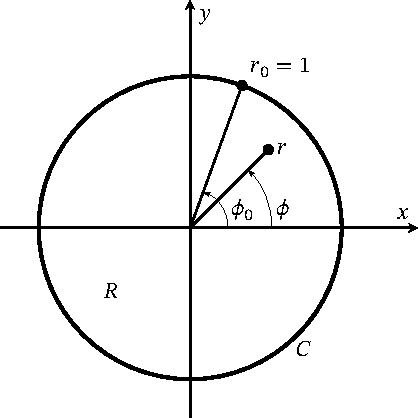
\includegraphics[width=0.7\linewidth]{figures/sample-figure-1.pdf}
\caption{A figure caption with math, Eq.~\eqref{eqn:1}: $z = (r,\phi)$ \cite{Lienhard2019b}\label{fig:1}}
\end{figure}

%%%%%%%%%%%%% end figure %%%%%%%%%%%%%%%%%%%%%%%%%%%%%%%%%%%%%%%%%%%%%%%%%%%%%%


%%%%%%%%%%%%%%%%%%%%%%%%%%%%%%%%%%%%%%%%%%%%%%%%%%%%%%%%%%%%%%%%%%%%%%%%%%%%%%%
\section{Tables and Figures}

Table \ref{tab:1} is an example of a simple table. Table captions should be placed above tables.
The class loads the \texttt{array} and \texttt{dcolumn} packages which provide extended capabilities for columns in the \texttt{tabular} environment (used in Tables \ref{tab:2} and \ref{tab:3}). Table~\ref{tab:3} is coded to have exactly the width of a text column.

The \texttt{booktabs} package \cite{fear} is loaded (and customized) to provide versions of \verb|\toprule|, \verb|\midrule|, and \verb|\bottomrule| appropriate to ASME-style tables.

Table~\ref{tab:4} shows a table that spans both text columns. Figure~\ref{fig:2} shows a figure spanning both columns. Two column tables and figures will always float to the top of a later page. Subframes in figures, such as  Fig.~\ref{fig:interior-region}, may be referenced individually.

Text in the figures should be checked for legibility at either single-column width (about 83~mm) or full-column width (about 170~mm).  Figure captions should be placed below figures. Images in figures are handled by the standard \texttt{graphicx} package.

Landscape figures and tables may be produced at full-page size by putting \verb|\usepackage[figuresright]{rotating}| in your \texttt{.tex} file's preamble and using the \texttt{sidewaystable*} and \texttt{sidewaysfigure*} environments~\cite{fairbairns}.


%%%%%%%%%%%%%%%%%  begin two column figure  %%%%%%%%%%%%%%%%%%%%%%%%%%%%%%%%%%%%

\begin{figure*}[t]
\begin{subfigure}[t]{0.5\textwidth} % You will get same result using \begin{minipage}[t]{0.5\textwidth}
\vbox{
\vspace*{1.7em}
\centering{
  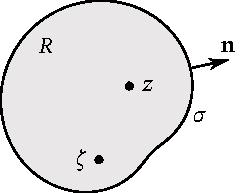
\includegraphics{figures/sample-figure-2a.pdf}
}
\vspace*{1.7em}
}
\subcaption{\label{fig:interior-region}}
\end{subfigure}%
%%%%%%%% don't leave a break here
\begin{subfigure}[t]{0.5\textwidth} % You will get same result using \begin{minipage}[t]{0.5\textwidth}
\centering{
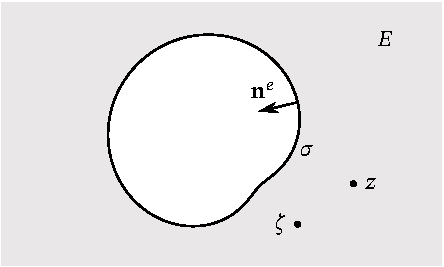
\includegraphics{figures/sample-figure-2b.pdf}
\subcaption{\label{fig:exterior-region}}
}\end{subfigure}%
\caption{A figure with two subfigures: \subref{fig:interior-region} interior region, and \subref{fig:exterior-region} exterior region \cite{Lienhard2019b}\label{fig:2}}
\end{figure*}

%%%%%%%%%%%%%%%  end two column figure  %%%%%%%%%%%%%%%%%%%%%%%%%%%%%%%%%%%%%%%%


%%%%%%%%%%%%%%%%%%%%%%%%%%%%%%%%%%%%%%%%%%%%%%%%%%%%%%%%%%%%%%%%%%%%%%%
\section{Reference Formatting with \texttt{asmejour.bst}}

The {\upshape\texttt{asmejour.bst}} \hologo{BibTeX} style follows the reference styles observed in ASME journals in 2020.\footnote{\texttt{asmejour.bst} is intended as a replacement for the older style \texttt{asmems4.bst}, which does not follow ASME's current reference formats or support DOI and URL.} The vast majority of published references are to journal papers and books. Examples for these and many other entry types are given in the \texttt{asmejour-sample.bib} file, which is part of this distribution. Citations and references are managed by the standard \texttt{natbib} package.
Nevertheless, a few comments are necessary.

\subsection{Capitalization of Titles} ASME's bibliography style requires that titles be in title case. The first letters of principal words are capitalized. This must be done when writing the \texttt{.bib} file.
%(ASME capitalizes ``With'', but not other prepositions).

\subsection{Hyperlinked Titles or Paper Numbers} When the entries \verb|@article{..|, \verb|@book{..|, \verb|@inbook{..|, \verb|@incollection{..|, \verb|@proceedings{..|, or \verb|@techreport{..| include \verb|doi={..}|, the document title, paper number, or report number will be hyperlinked to that doi number, and the doi number will not be printed. If no doi is included, but a url or eprint is included, then the title will be hyperlinked to that url or eprint. To display the doi (or the url or eprint when no doi is given), put it into the \verb|note={..}| field (using \verb|\doi{..| or \verb|\url{..| ):
\begin{quote}
\verb|note = {\doi{10.1115/1.4042912}}|
\end{quote}
Include doi numbers in references whenever possible.

%%%%%%%%%%%%%%% begin simple table %%%%%%%%%%%%%%%%%%%%%%%%%%%%%%%%%%%%%%%%%%%%%

%% captions go above tables

\begin{table}[t]
\caption{A simple table\label{tab:1}}
\centering{%
\begin{tabular}{l l r}
\toprule
Experiment & $u$ [m/s] & $T$ [\textdegree C] \\
\midrule
Run 11 & 12.5 & 103.4 \\
Run 12 & 24   & 68.3 \\
\bottomrule
\end{tabular}
}%
\end{table}

%%%%%%%%%%%%%%%%%  end table  %%%%%%%%%%%%%%%%%%%%%%%%%%%%%%%%%%%%%%%%%%%%%%%%%%%

%%%%%%%%%%%%%%% begin more complicated table %%%%%%%%%%%%%%%%%%%%%%%%%%%%%%%%%%%%

\begin{table}[t]
\caption{Table with more complicated columns}\label{tab:2}%
\centering{%
\begin{tabular}{!{\hspace*{0.5cm}} >{\raggedright\hangindent=1em} p{3cm} d{3} @{\hspace*{1cm}} d{3} !{\hspace*{0.5cm}}}
\toprule
Experiment & \multicolumn{1}{c@{\hspace*{1cm}}}{$u$ [m/s]} & \multicolumn{1}{c!{\hspace*{0.5cm}}}{$T$ [\textdegree C]} \\
\midrule
The first experiment we ran this morning   & 124.3     &   68.3  \\
The second experiment we ran this morning  &  82.50    &  103.46 \\
Our competitor's data                      &  72.321   &  141.384\\
\bottomrule
\end{tabular}
}%
\end{table}

%%%%%%%%%%%%%%%% end table  %%%%%%%%%%%%%%%%%%%%%%%%%%%%%%%%%%%%%%%%%%%%%%%%%%%%%

\subsection{eprint Support} Elementary support for \texttt{eprint} numbers is included, either hyperlinking or generating a url at the end of the citation. The \texttt{archive} type may be specified using the macros \texttt{arxiv, googlebooks, hndl, jstore, oclc}, or \texttt{pubmed} (e.g., \texttt{archive=hndl},  \textit{without} braces). Both \texttt{eprint} and \texttt{archive} fields \textit{must} be given. Other root urls may be invoked using \verb|archive = {http://another.url.org/}|.

\subsection{Online Sources} A bibliography field \verb|@online{..| is included for citation of online sources, such as web pages. A \texttt{url}, \texttt{doi}, or \texttt{eprint} with \texttt{archive} should be included. See the examples of use in the \texttt{asmejour-sample.bib} file.

\subsection{Date Accessed} The \verb|urldate={..}| field may be used to provide the date on which a given url was accessed. By default, the text printed will be \texttt{accessed `date',}. The word ``accessed'' may be changed using the \verb|urltype={..}| field.

\subsection{Conference Location and Date} For the entry types \verb|@inproceeedings{..| and \verb|@proceeedings{..|, you may include \verb|venue={..}| and \verb|eventdate={..}| to specify the city and the date of a conference. Omit \verb|address={..}| if \verb|venue={..}| is used.

\subsection{Version Number\protect\footnote{Footnotes can appear in \texttt{\string\section} commands. However, when the \texttt{[lineno]} option is used either: i) write \texttt{\string\protect\string\footnote\{..\}}; or ii) include the optional argument, as in \texttt{\string\section[Foo]\{Foo\string\footnote\{..\}\}}.\label{ftnt:3}}}
The \verb|version={..}| field may be used with \verb|@book|, \verb|@online|, and \verb|@manual|. By default, the text will read \texttt{Version `number'} as in Refs.~\cite{sharpe1,sharpe2},  but different wording may be selected using the \verb|versiontype={..}| field, to have ``Revision''  or something similar, as in Ref.~\cite{GSL}. ASME often puts the version in the title, as in Refs.~\cite{dlmf, texshop}, so I've left the final decision for discussion between the authors and the copy editor.

\subsection{Articles in Collections} In addition to the standard entry, \verb|@incollection{..|, an entry  \verb|@inserialcollection{..| is defined for serials in which each volume has a different title. See the \texttt{asmejour-sample.bib} file for discussion and compare Ref.~\cite{clauser56} to Ref.~\cite{DKE70}.

%%%%%%%%%%%%%%%%%%%%%%%%%%%%%%%%%%%%%%%%%%%%%%%%%%%%%%%%%%%%%%%%%%%%%%%%%%%%%%%%%
\section{More on Math}
Math italics are used for roman and lower-case greek letters by default.  If you want an upright letter in math, you can use the relevant math alphabet, e.g., \verb|\mathrm, \mathbf, \mathsf|:
\begin{equation}\label{eqn:newton2}
\vec{F} = m \vec{a} \quad\textrm{or}\quad \vec{\mathrm{F}} = m \vec{\mathrm{a}} \quad\textrm{or}\quad \mathbf{F} = m \mathbf{a} \quad\textrm{or}\quad \vec{\mathsf{F}} = m \vec{\mathsf{a}}
\end{equation}

ASME typesets vectors in upright bold, like the third instance in Eq.\ \eqref{eqn:newton2}, and sets matrices in bold italic. In the next equation, $\mathbf{w}$ is a vector and  $\bm{J}_1$ is a matrix:
\begin{equation}\label{eqn:dw}
d\mathbf{w} =
   \begin{pmatrix}
 	du \\ dv
   \end{pmatrix} =
   \underbrace{\begin{pmatrix}
	 \partial u/\partial x &  \partial u/\partial y \\
	 \partial v/\partial x &  \partial v/\partial y
   \end{pmatrix}}_{=\,\bm{J}_1}  \begin{pmatrix}
 	dx \\ dy
   \end{pmatrix}
\end{equation}

To get additional symbols in bold math, you can use the \verb|\bm{..}| macro from the \texttt{bm} package, which is loaded by the class
\begin{equation}
\mathbf{u}_r = u_r\bm{\hat{\textbf{\i}}}+v_r\bm{\hat{\textbf{\j}}}+w_r\bm{\hat{\textbf{k}}}
\end{equation}
or, \textit{very} rarely, \verb|\mathversion{bold}| for an entire equation:
\mathversion{bold}\begin{equation}
S = k \ln w = k \ln \biggl(\frac{N!}{\prod_i N_i!}\biggr)
\end{equation}
\mathversion{normal}% avoid extra line break with %

In most cases, long equations can be kept below the column width by using one of the multiline equation environments defined by \texttt{amsmath},
such as \texttt{align}, \texttt{split}, or \texttt{multline}~\cite{amsmath}. The following equation is set with the \texttt{multline} environment:
\begin{multline}
\frac{\partial}{\partial t}\left[\rho\Bigl(e + \lVert\mathbf{u}\rVert^2\mspace{-3mu}\big/2\Bigr)\right]  + \nabla\cdot\left[\rho\Bigl(h + \lVert\mathbf{u}\rVert^2\mspace{-3mu}\big/2 \Bigr)\mathbf{u}\right]\\
 ={}-\nabla \cdot \mathbf{q} +  \rho \mathbf{u}\cdot\mathbf{g}+ \frac{\partial}{\partial x_j}\bigl(d_{ji}u_i\bigr) + \dot{Q}_v\label{eqn:energy}
\end{multline}
An example using \texttt{align} appears in Appendix~\ref{app:zetafunction}.

An alternative solution may be to set large equations into two-column-wide tables or figures. While a package exists for setting equations that span two columns (\texttt{widetext.sty}), that code is erratic in relation to floats and page breaks.

\subsection{\texttt{newtxmath} and \texttt{mathalpha}} The \texttt{newtxmath} package~\cite{sharpe1}, loaded by default, includes a large number of options for mathematics, most of which can be called as options to \verb|\documentclass|. For example, the \texttt{upint} option of \texttt{newtxmath} selects upright integral signs (rather than slanted integral signs):
\begin{quote}
\verb|\documentclass[upint]{asmejour}|.
\end{quote}
The option \verb|subscriptcorrection| improves the spacing of math subscripts. Math options are discussed further in the \texttt{asmejour-template.tex} file.

In addition, many options for calligraphic, script, and fraktur fonts are available through the \texttt{mathalfa} package, which is also loaded. These may be invoked, for example, as
\begin{quote}
\verb|\documentclass[mathalfa=cal=euler]{asmejour}|
\end{quote}
which selects the Euler font for \verb|\mathcal|, as in $A \in \mathcal{P}(A)$. %($\mathcal{T}_1 \subset \mathcal{T}_2$)
To see all the font options, refer to the \texttt{mathalfa} documentation \cite{sharpe2}.

The class is designed for use with \texttt{newtxmath} and does not support the \texttt{unicode-math} package.

%% Dealing with complicated math in a section heading: optional argument of \section provides the pdfbookmark
%%    without losing characters or producing warnings/errors. Note that bookmark can include simple math and \eqref{..}.
%% newtxmath provides the option for upright Greek letters as \upomega (vs. \omega), etc.
\subsection[Math in a Section Heading: \omega\cdot U=0]{Math in a Section Heading: $\tilde{\upomega}\cdot\hat{\mathrm{U}}=0$}

To include complicated math in a section heading without producing bookmark-related errors, use the optional argument of \verb|\section| to create the pdfbookmark. The heading above was set with the following command:
\begin{quote}\raggedright
\verb|\subsection[Math in a Section Heading:|
\hspace*{1em}\verb|\omega\cdot U=0]{Math in a Section Heading:|
\hspace*{1em}\verb|$\tilde{\upomega}\cdot\hat{\mathrm{U}}=0$}|
\end{quote}
Note that bookmarks can include simple math. Also note that \texttt{newtxmath} provides the option to obtain upright Greek letters, such as \verb|\upomega| (vs.\ \verb|\omega|).


\subsection{Units and Nomenclature} ASME requires SI units. U.~S.\ style units may be follow in parentheses. Be sure to put your symbols into the nomenclature list, including the SI units.


%%%%%%%%%%%%%%%%%%%%%%%%%%%%%%%%%%%%%%%%%%%%%%%%%%%%%%%%%%%%%%%%
\section{Additional Options for \texttt{asmejour.cls}}
%The class accepts a number of options in addition to those already described.

\subsection{Lists of Figures and Tables} A list of figures and a list of tables are generated automatically as the last page.  To omit these lists, use the option \texttt{[nolists]}.

\subsection{Final Column Balancing} The option \texttt{[balance]} invokes the the \texttt{flushend} package~\cite{tolusis}.
This package will attempt to give equal height to the two columns on the last page. The performance of this package is sometimes inconsistent (with odd page layout or, very rarely, errors), so use this option with caution.

\subsection{Line Numbers} The option \texttt{[lineno]} invokes the the \texttt{lineno} package~\cite{bottcher}.  This will produce line numbers in the margins. You must run \LaTeX\ \textit{twice} for proper placement of the numbers. The \texttt{lineno} package is not compatible with the \texttt{flushend} package that makes final short columns the same height. Balancing is disabled when this option is called. See the documentation of the \texttt{lineno} package for further commands to control line numbering. See footnote~\ref{ftnt:3} with regard to footnotes in section headings while this option is in~effect. The abstract, tables, captions, and footnotes will not be numbered.

\subsection{Changing the Footer Text}\label{sec:footer} The option \texttt{[nofoot]} will omit everything other than a page number from the page footer.  The option \texttt{nocopyright} will omit the ASME copyright from the first page footer. The command \verb|\PreprintString{..}| replaces the words \textsf{PREPRINT FOR REVIEW}. The left and right preprint strings can be changed separately using an optional argument: \verb|\PreprintString{..}[L]| and \verb|\PreprintString{..}[R]|.
The final paper number may be added to the page number using \verb|\PaperNumber{..}|.

The footers are all generated with the \texttt{fancyhdr} package~\cite{oostrum}, and you can change them using the commands of that package.

\subsection{Vertical Space on Title Page} The space between the author/title/abstract block and the main text defaults to 12.5~mm. Infrequently, a different value may be desirable.  The space can be changed using \verb|\AbstractSep{..}|, where the argument is a \LaTeX\ dimension with units (e.g., 5mm).

\subsection{Federal Copyright Notices} Several types of copyright statement can be placed an unnumbered footnote on the first page. Use the option \texttt{[govt]} when all authors are federal employees, \texttt{[govtsome]} when some authors are federal employees, and \texttt{[contractor]} when the authors are federal contractors.

\subsection{Archivability:~PDF/A} Compliance with PDF/A standards can be enabled using the option \texttt{[pdf-a]}
when running with \hologo{pdfLaTeX}. The
default setting is for PDF/A-3u with sRGB OutputIntent (\texttt{sRGB.icc}). If levels 1b, 2b, 2u, or 3b are preferred, use the
options \texttt{[pdfapart=1 or 2 or 3]} and  \texttt{[pdfaconformance=b or u]}. Note that accessible
conformance~(\texttt{a}) is not currently possible with \LaTeX.

\subsection{Superiors Font} The \texttt{newtxtext} package includes a superiors font (numbers and letters) for use in footnote markers and superscripts. The option \texttt{[nodefaultsups]} enables this font. (The corresponding author mark in the author block will not change.)

\subsection{Typewriter Font Options} This font is the sans-serif, monospaced font \texttt{inconsolata}. By default, the word spacing is variable, but option \texttt{[mono]} ends this behavior. A slashed zero is the default; option \texttt{[var0]} removes the slash. Option \texttt{[hyphenate]} enables hyphenation of the typewriter font.%(This option is not available if the \texttt{[fontspec]} option is used.)


%%%%%%%%%%%%%%%%%%%  begin linewidth table  %%%%%%%%%%%%%%%%%%%%%%%%%%%%%%

\begin{table}[t]
\newcolumntype{C}{>{$}c<{$}} % math-mode version of "c" column type, from array package
\caption{\label{tab:3}Table at full column width with columns in math mode}
\begin{tabular*}{\linewidth}{@{\extracolsep{\fill}}CCCC@{\extracolsep{\fill}}}
\toprule
X_{z} & X_{c} & X_{c,m} & X_{c,2}\rule{0pt}{8pt}\\
 3.92069  & 5.70943 & 6.32429 & 7.08757\\[2pt]
\varepsilon (T_1)  & \varepsilon^i (T_1) & \varepsilon^i (T_m) & \alpha (T_1, T_2)\\
0.7258 & 0.6237 & 0.6807 & 0.7964 \\[2pt]
q_\textrm{gray}  & q_\textrm{int, $T_1$} & q_\textrm{int, $T_m$} & q_\textrm{exact}\\
400.2 & 462.1 & 371.0 & 371.8 \\
\bottomrule
\end{tabular*}
\end{table}

%%%%%%%%%%%%%%%%%%%%  end linewidth table %%%%%%%%%%%%%%%%%%%%%%%



%%%%%%%%%%%%%%% begin two column table %%%%%%%%%%%%%%%%%%
\begin{table*}[t]
\caption{A table spanning two columns}\label{tab:4}%
\centering{%
\begin{tabular*}{0.8\textwidth}{@{\hspace*{1.5em}}@{\extracolsep{\fill}}ccc!{\hspace*{3.em}}ccc@{\hspace*{1.5em}}}
\toprule
\multicolumn{1}{@{\hspace*{1.5em}}c}{$x$\rule{0pt}{8pt}} &
\multicolumn{1}{c}{$\textrm{erf}(x)$} &
\multicolumn{1}{c!{\hspace*{3.em}}}{$\textrm{erfc}(x)$} &
\multicolumn{1}{c}{$x$} &
\multicolumn{1}{c}{$\textrm{erf}(x)$} &
\multicolumn{1}{c@{\hspace*{1.5em}}}{$\textrm{erfc}(x)$} \\ \midrule
0.00 & 0.00000 & 1.00000 & 1.10 & 0.88021 & 0.11980 \\
0.05 & 0.05637 & 0.94363 & 1.20 & 0.91031 & 0.08969 \\
0.10 & 0.11246 & 0.88754 & 1.30 & 0.93401 & 0.06599 \\
0.15 & 0.16800 & 0.83200 & 1.40 & 0.95229 & 0.04771 \\
0.20 & 0.22270 & 0.77730 & 1.50 & 0.96611 & 0.03389 \\
0.30 & 0.32863 & 0.67137 & 1.60 & 0.97635 & 0.02365 \\
0.40 & 0.42839 & 0.57161 & 1.70 & 0.98379 & 0.01621 \\
0.50 & 0.52050 & 0.47950 & 1.80 & 0.98909 & 0.01091 \\
0.60 & 0.60386 & 0.39614 & 1.82\makebox[0pt][l]{14} & 0.99000 & 0.01000 \\
0.70 & 0.67780 & 0.32220 & 1.90 & 0.99279 & 0.00721 \\
0.80 & 0.74210 & 0.25790 & 2.00 & 0.99532 & 0.00468 \\
0.90 & 0.79691 & 0.20309 & 2.50 & 0.99959 & 0.00041 \\
1.00 & 0.84270 & 0.15730 & 3.00 & 0.99998 & 0.00002 \\
\bottomrule
\end{tabular*}
}%
\end{table*}
%%%%%%%%%%%%%%%% end two column table %%%%%%%%%%%%%%%%%%%

%%%%%%%%%%%%%%%%%%%%%%%%%%%%%%%%%%%%%%%%%%%%%%%%%%%%%%%%%%%%%%%%%%%%%%
\section{Conclusions}
The class \texttt{asmejour} and associated files are for typesetting preprints in the style of ASME journals.
Documentation is provided in this file and by comments in the \texttt{.tex} source code. Examples of references are shown in the \texttt{asmejour-sample.bib} file.  The \texttt{asemjour.bst} file produces references following ASME's current formats.  The code is compatible with both {\hologo{pdfLaTeX}} and \LuaLaTeX. This package is not a publication of ASME and is offered at no cost under the terms of the \href{https://ctan.org/license/mit}{MIT license}.

\begin{enumerate}
\item First conclusion
\item Second conclusion
\item Third conclusion
\end{enumerate}


%%%%%%%%%%%%%%%%%%%%%%%%%%%%%%%%%%%%%%%%%%%%%%%%%%%%%%%%%%%%%%%%%%%%%%
\section*{Acknowledgment} %% ASME requests this exact spelling, singular.

Acknowledge individuals, institutions, or companies that supported the authors in preparing the work. Those mentioned might have provided technical support, insightful comments or conversations, materials used in the work, or access to facilities.


%%%%%%%%%%%%%%%%%%%%%%%%%%%%%%%%%%%%%%%%%%%%%%%%%%%%%%%%%%%%%%%%%%%%%%
\section*{Funding Data}
\begin{itemize}
\item U.S.\ Department of Heat Transfer, Office of Important Ideas (DOHT-OII Award No.\ 3.14159265)
\end{itemize}


%%%%%%%%%  NOMENCLATURE  %%%%%%%%%%%%%%%%%%%%%%%%%%%%%%%%%%%%%%%%%%%%%
%%
%% Name of nomenclature can be changed using an optional argument to the environment.
%%
%% \EntryHeading{Greek Letters}
%% \entry{symbol}{definition}
%%
%% Must run latex twice to align the columns.

\begin{nomenclature}

\entry{$\overline{h}$}{average heat transfer coefficient (W m$^{-2}$ K$^{-1}$)}
\entry{$k$}{thermal conductivity (W m$^{-1}$ K$^{-1}$)}
\entry{$\mathbf{q}$}{heat flux vector (W m$^{-2}$)}

\EntryHeading{Greek Letters}
\entry{$\alpha$}{thermal diffusivity (m$^2$ s$^{-1}$)}
\entry{$\nu$}{kinematic viscosity (m$^2$ s$^{-1}$)}

\EntryHeading{Dimensionless Groups}
\entry{Pr}{Prandtl number, $\nu/\alpha$}
\entry{Sc}{Schmidt number, $\nu/\mathcal{D}_{1,2}$}

\EntryHeading{Superscripts and Subscripts}
\entry{b}{bulk value}
\entry{$\infty$}{free stream value}

\end{nomenclature}


%%%%%%%%%%%%%%%  APPENDICES  %%%%%%%%%%%%%%%%%%%%%%%%%%%%%%%%

%% Note that appendices will be "numbered" A, B, C, ... etc. Use \section, not \section*
%% Subsections need not be numbered, use \subsection*
%% The equation counter is reset for each appendix
%% Figures will be numbered consecutively

\appendix   %%% starting appendices

%%%%%%%%%%%%%%%%%%%%%%%%%%%%%%%%%%%%%%%%%%%%%%%%%%%%%%%%%%%%%%%%%%%%%%
\section{Incomplete Zeta Function~\cite{Lienhard2019c}\label{app:zetafunction}}

This text is just for illustration. The radiation fractional function may be written in terms of the incomplete zeta function for convenience:
\begin{align}
f(\lambda T)  = {}&  \frac{1}{\sigma T^4} \int_0^\lambda\frac{2\pi h c_o^2}{\lambda^5 \left[ \exp (h c_o/k_B T \lambda) - 1\right] } \, d\lambda \\
 = {}&  \frac{1}{\sigma T^4}\frac{2\pi k_B^4 T^4}{h^3c_o^2}\int^\infty_{c_2/\lambda T}\frac{t^3}{e^t -1}\, dt\label{eqn:zeta}
\end{align}
When $\lambda T \rightarrow \infty$, $f = 1$ and the last equation yields the well-known result
\begin{equation}
 {\sigma T^4} =\frac{2\pi k_B^4 T^4}{h^3c_o^2} \underbrace{\int_0^\infty \frac{t^3}{e^t - 1} \, dt}_{\equiv\mspace{2mu} \zetaup(4)\Gamma(4)}
\end{equation}
where the Gamma function $\Gamma(4) = 3!$ and the Riemann zeta function, $\zetaup(4)$, has the indicated integral representation \cite[\S13.12]{ww1927}.  A classical result due to Euler \cite{euler1740} gives $\zetaup(4) = \pi^4/90$ (see also \cite[\S167]{euler1748}), from which we recover the usual definition of the  Stefan-Boltzmann constant, $\sigma$.


%%%%%%%%%%%%%%%%%%%%%%%%%%%%%%%%%%%%%%%%%%%%%%%%%%%%%%%%%%%%%%%%%%%%%%
\section{Language Support}

ASME publishes in English, but the \texttt{babel} package is loaded for users who may wish to include other languages.
For example, an author might wish to include an appendix that provides the abstract in another language.

When more than one language option is included in \verb|\documentclass[..]{asmejour}|, English will be
assumed to be the main language of the document. (To choose a different main language, set \texttt{[main=..]}).
If no language options are given, the package defaults to English.  As an example, a passage in French is
shown in \selectlanguage{french}\appendixname~\ref{app:fourier}\selectlanguage{english}.

The standard caption and section names will follow \texttt{babel}'s dictionary for primary languages other than English.  Users may additionally change ``Keywords'', ``Nomenclature'', and  ``Corresponding author'' by renewing the commands \verb|\keywordname|, \verb|\nomname|, and \verb|\CAwords|. Changes to the page footer were described in Sec.~\ref{sec:footer}. The pdf bookmark for ``Appendices'' by be changed by renewing \verb|\appendicesname|.

The font encoding is set to T1 and utf-8 input is supported:
%% If you have trouble with the next line (or the French text that follows), your file may not be saved in utf-8 format. You can delete these lines to resolve the issue.
\typeout{If you have trouble with the next line, your file may not be saved in utf-8 format. You can delete that line to resolve the issue.}
àáâäæãåā  èéęëêēė  îïíīįì ôöòóœøōõ ûüùúū çćč ł ñń ßśš ÿ žźż

No effort has been made to support customization of language-specific fonts (some fonts can be implemented using the \texttt{substitutefont} package~\cite{milde}). The bibliography style, \texttt{asmejour.bst}, is designed in English and aimed at \texttt{BibTeX}.  Multilingual bibliographies can be supported using \texttt{BibLaTeX}.

%%%%%%%%%%%%%%%%%%%%%%%%%%%%%%%%%%%%%%%%%%%%%%%%%%%%%%%%%%%%%%%%%%%%%%
\selectlanguage{french}
\section{Discours Préliminaire de Fourier}\label{app:fourier}
Les causes primordiales ne nous sont point con­nues; mais elles sont assujetties à des lois simples et constantes, que l'on peut découvrir par l'obser­vation, et dont l'étude est l'objet de la philosophie naturelle.

La chale ur pénètre, comme la gravité, toutes les substances de l'univers, ses rayons occupent toutes les parties de l'espace. Le but de notre ouvrage est d'exposer les lois mathématiques que suit cet élé­ment. Cette théorie formera désormais une des branches les plus importantes de la physique gé­nérale~\cite{fourier1822}.

\selectlanguage{english}


%%%%%%%%%%%%%  BIBLIOGRAPHY  %%%%%%%%%%%%%%%%%%%%%%%%%%%%%%%%%%%%%%%

% \nocite{*} %% <=== delete this line - unless you wish to typeset the entire contents of your .bib file.

% \bibliographystyle{asmejour}   %% .bst file that follows ASME journal format. Do not change.

% \bibliography{asmejour-sample} %% <=== change this to name of your bib file

%%%%%%%%%%%%%%%%%%%%%%%%%%%%%%%%%%%%%%%%%%%%%%%%%%%%%%%%%%%%%%%%%%%%%%

%% To omit final list of figures and tables, use the class option [nolists]

\end{document}
